%\documentclass[11pt, leqno]{article}
\documentclass[11pt]{article}
\usepackage{amsmath}
\usepackage{amsthm}
\usepackage{amssymb}
\usepackage{amsfonts}
\usepackage{longtable}
\usepackage{epsfig}
\usepackage{color}



\usepackage[utf8]{inputenc}
\usepackage[margin=1in]{geometry}
\usepackage{graphicx}
\usepackage{kotex}
\usepackage{mathtools}
\usepackage{setspace}
\usepackage{caption}
\usepackage{subcaption}
\usepackage{float}
\usepackage[table,xcdraw]{xcolor}
\usepackage{multirow}
\usepackage{afterpage}

\renewcommand{\baselinestretch}{1.2}
\newcommand{\mydoublespace}{\setlength{\baselineskip}{22pt}}
\hoffset=-25.5 truemm \voffset=-26. truemm
\setlength{\textheight}{8.5 true in} \setlength{\textwidth}{6.5true
in} \setlength{\oddsidemargin}{1.0 true in}
\setlength{\evensidemargin}{.25 true in}
\setlength{\topmargin}{0.615 true in} \setlength{\baselineskip}{1.75
\baselineskip}
%\def\theequation{\thesection.\arabic{equation}}
%\def\theequation{\thesection.\arabic{equation}}
\newtheorem{thm}{Theorem}[section]
\newtheorem{lm}{Lemma}[section]

%\mydoublespace
\newtheorem{lemma}{Lemma}
\newtheorem{theorem}{Theorem}
\newtheorem{proposition}{Proposition}
\newtheorem{assumption}{Assumption}
\newtheorem{remark}{Remark}
\newtheorem{corollary}{Corollary}
\newtheorem{claim}{Claim}

\renewcommand{\floatpagefraction}{0.1}
\renewcommand{\labelitemi}{$\bullet$}
\renewcommand{\labelitemii}{$\cdot$}
\renewcommand{\labelitemiii}{$\diamond$}
\renewcommand{\labelitemiv}{$\ast$}





%============================================================================
% Title and Abstract
%============================================================================

\begin{document}

\begin{center}
{\bf\LARGE A Neural Network-based Clustering Methods for Statistical Arbitrage}
\vspace{.5cm}\\
 Dongwuk Kim, Seungkyu Kim, Chang Kyeom Kim \\
Department of Statistics, Seoul National University, Seoul, 08826,
Korea\\
\end{center}


\begin{abstract}
This paper aims to propose the deep neural network-based clustering scheme that can be applied to boost the performance of statistical arbitrage strategies, such as the mean-reversion strategy. The performance of the `deep clustering' model was compared against the traditional k-means clustering method, as well as the vendor-classified cluster, with the Sharpe ratio as a measure of performance. Although the deep clustering-based model outperforms that of k-means clustering, there still is room for improvement, which can be interesting future works.
\end{abstract}

\noindent{\bf Key words}: Mean-reversion strategy, statistical arbitrage, deep learning, autoencoder, k-means clustering.


%============================================================================
% Section 1: Introduction
%============================================================================

\section{Introduction}

In this study, we aim to develop a neural network-based clustering method, which will be utilized in the field of statistical arbitrage strategy called ``mean-reversion". The mean-reversion strategy is one of the trends of the financial industries to formulate a portfolio in the securities market. %(여기에 2줄 정도 다른 논문 citation과 함께 내용 덧붙여주세요!)

Meanwhile, in the past few years, quite a few clustering methods that revolve around deep learning framework were advocated in favor of the previous nonparametric models. These methods can be categorized into autoencoder-based approaches such as the `deep embedded network' (Xie et al., 2016), convolutional neural network(CNN)-based approach, or generative adversarial model(GAN)-based approach. A survey of these aforementioned methodologies can be found in Min et al. (2018). Moreover, the success of the deep clustering models which classifies various data, such as  Bojanowski and Joulin (2017) and Caron et al. (2018), with the visual data. However, to our knowledge, we could not find a deep neural network-based clustering approach that was applied to the statistical arbitrage strategy in the literature. Therefore, this paper is a contribution in the sense that this approach can outperform the traditional clustering methods in combination with the mean-reversion strategy.

This paper is organized as follows. Section 2 reviews the basic mean-reversion strategy that was adopted when developing the model. Section 3 proposes a clustering method and its result when the mean-reversion strategy is combined with k-means clustering. Section 4 discusses the autoencoder-based deep model and its details, as well as its performance. Section 5 provides the concluding remarks.



%============================================================================
% Section 2
%============================================================================


\section{Mean-reversion Strategy}
In this section, we briefly review the notion of mean-reversion strategy. A mean-reversion strategy refers to...




%============================================================================
% Section 3
%============================================================================

\section{A Statistical Arbitrage with Nonparametric Clustering}
In this section, ...


%============================================================================
% Section 4
%============================================================================

\section{A Statistical Arbitrage with Deep Learning}
In this section, we propose a neural network-based model that concentrates on clustering the corporations in the securities market, which has the best performance when making a portfolio with the mean-reversion strategy. The subsequent subsections portray the process and behind-the-scenes decisions when constructing the model.

\subsection{Model Construction}
In the past years, numerous deep models were advocated, which claims to effectively provide a solution to the problem of clustering unlabeled datasets in the literature. To illustrate, the Deep Embedded Clustering proposed by Xie et al. (2016), is one of the pioneers of such an approach. They proposed the clustering method, which combines the existing clustering model and the power of deep models. The gist of this model is that it has two training phases, and can be summarized as Figure \ref{DEC}: 

\begin{itemize}
    \item \textbf{Phase 1.} Construct an autoencoder that 'embeds' the input to the lower-dimensional feature space. This approach is taken place in order to escape from the 'curse of dimensionality' problem. Also, it is to find a nonlinear map that finds the parameters necessary for the k-means clustering to operate correctly.
    \item \textbf{Phase 2.} Conduct the k-means algorithm to obtain the cluster centers, and compute the 'auxiliary' distribution based on t-distribution with the values obtained from Phase 1. This will be considered as the 'pseudo-true' label and will be compared against the 'target distribution' also computed from the values obtained from above by computing the KL divergence between the two.
\end{itemize}

\begin{figure}
    \centering
    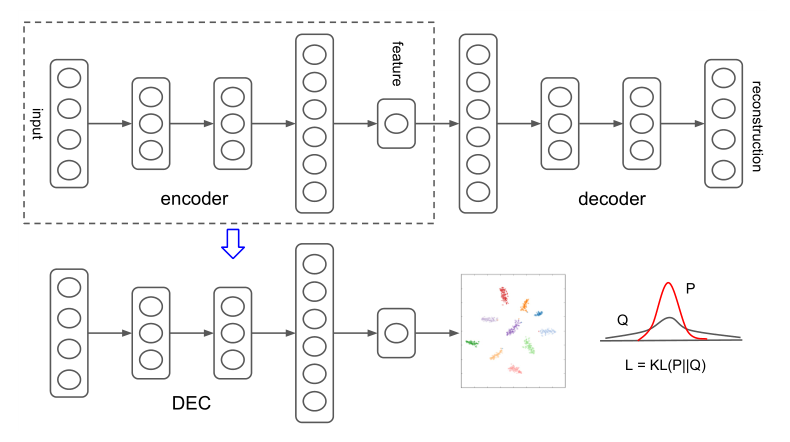
\includegraphics[width=14cm]{images/dec-model.png}   
    \caption{Outline of the deep embedded clustering (Xie et al, 2016.)}
    \label{DEC}
    \vspace*{-5mm}
\end{figure}

At a glance, this approach is lucrative in a sense that it attempts to cluster from the feature space, which may significantly reduce the computational burden. Also, this network can be useful as it exploits the advantage of supervised learning by formulating 'auxiliary distribution,' which acts as a true label. Albeit these advantages, we opted against this approach in the end.

One of the limitations of this model is that it heavily relies on another nonparametric clustering mechanism to cluster the input itself. In other words, roughly speaking, it can be interpreted as a 'fancier' version of clustering after applying dimension reduction techniques, such as principal component analysis. What we intend to design is the clustering model that directly assigns an input to a specific cluster without any help from other clustering models. At the same time, we were motivated by the autoencoder approach, which forms a building block for the clustering algorithm to function. Therefore, in this paper, we intend to create an autoencoder-like network which outputs cluster information within the network.

Two justifications can be made regarding this approach. To start, the ultimate goal to accomplish is to build a portfolio that maximizes the profit, while the cluster of corporations can be considered as one of the chunks while generating the portfolio. This implies that despite the accuracy being one of the priorities, it does not exceed that of gaining more profit. Furthermore, this model does not require a two-phase training scheme and is designed to output the cluster information after filtering through the encoder part of the network. With this approach, the computation cost may be reduced, as the resource is severely limited when it comes to training `deeper' models.

To depict our model, we first design a custom loss function as a weighted sum of two separate functions as below:
\begin{equation}
    (\text{Loss}) = \alpha \times \text{(reconstruction loss)} + (1-\alpha) \times \text{(mean-reversion loss)},
\end{equation}

where $\alpha \in [0, 1]$. The loss above can not only serve the purpose to maximize the profit (mean-reversion loss) but can also stabilize the model (reconstruction loss). In other words, the reconstruction loss acts as a regularization term to prevent the model from overfitting. For the 'mean-reversion loss,' we adopt the Sharpe ratio of a given portfolio, defined as above in Section 2. Moreover, we employ the element-wise $\ell_2$ loss for the reconstruction loss.

Subsequently, we define the number of corporations $n$ that serves as an input, as well as the number of clusters $c$. This network is unique in the sense that the total number of clusters can vary. In fact, the number of clusters we assign is an upper bound of the total clusters, since the network has the freedom to not assign the corporations to one of the groups at all. This is one of the advantages over the classical k-means algorithm, as it must assign the inputs to a fixed number of clusters every time. However, the advantage of this design is undermined due to the number of inputs being fixed, contrary to the k-means clustering algorithm which does not have any restrictions regarding the number of inputs.

Because the original mean-reversion strategy utilizes the mean of the previous 5 trading days when forming the portfolio to reduce the volatility, the input of this network is a collection of $d$ days worth of return value of $n$ corporations, resulting in a tensor of $n \times d$ matrix. Similarly, the output of the encoder is $n \times c$ matrix, and the $p$-th row indicates the assignment probability of $p$-th corporation. As an illustration, if the company numbered A is assigned to the cluster 5, then, the (A, 5)-th element of the output matrix has the highest probability among the A-th row of such matrix. In addition, the encoder part of the model has one hidden layer with 128 nodes. The hidden layer is in place as an attempt to shrink the dimension before clustering. The decoder part is symmetric to that of the encoder. To summarize, the information of the encoder is as follows:

\begin{itemize}
    \item Input layer: $n \times d$ nodes.
    \item Hidden layer 1: 128 nodes, with 'relu' as a nonlinearity.
    \item Output layer: $n \times c$ nodes, with 'softmax' as a nonlinearity. \\
    This output is converted to a $n \times c$ matrix, each corporation is classified to the cluster which has the highest probability.
\end{itemize}

The following describes the tuning parameters and the optimizers:

\begin{itemize}
    \item Learning rate: $\eta \in \{ 0.001, 0.005, 0.01 \}.$
    \item Optimizer: RMSProp, Adam. \\
    The tuning parameters for other parameters of the optimizers were set to their defaults, namely the momentum $\rho = 0.9$ for RMSProp, and $\beta_1 = 0.9, \beta_2 = 0.999$ for Adam.
    \item $\alpha$ = 0.01.
\end{itemize}

If the learning rate is greater than 0.01, we have observed that the result diverges, therefore disregarded. Moreover, if the proportion of the reconstruction loss exceeds a certain threshold, we noticed that it tends to dominate the whole loss function and hampers the performance of the mean-reversion strategy, as seen in Figure \ref{bigalpha}. To elaborate, we can see that the Sharpe ratio highly fluctuates, as well as the net profit is significantly lower than that of the K-means or manual classification. This resulted in fixing $\alpha$ to a small value.

The performance of the model with various values of $n, c, d$ was provided at Figures \ref{deep result 1} to \ref{deep result 3}.

We observed that although the proposed model slightly outperforms the k-means approach in terms of the Sharpe ratio and the total profit, it suffers from lack of performance compared to the strategy based on the classification result provided by the vendor. This may be due to the following limitations of this network.

\begin{enumerate}
    \item \textbf{Fixed number of corporations.} \\
    The number of corporations constructing the portfolio was fixed to a certain number. This was an inevitable compromise since the number of input nodes must be fixed when constructing the deep model. However, in reality, the composition of the securities market may change each day. Also, the characteristics of each corporation may vary because of their actions, such as merging and acquisition. Therefore, if the whole dataset of the securities market were taken into account when training the model, the performance may have improved over the current one.
    \item \textbf{Limited role of the reconstruction loss.} \\
    The reconstruction loss was employed to prevent the model from overfitting, thus to stabilize the model. However, we have already seen that when the proportion of this reconstruction loss is large, then the performance is severely damaged. Therefore, re-purposing the decoder part as a different prediction model, such as a model that predicts the direction(sign) of the one-day-ahead return, can be an intriguing future work.
    \item \textbf{Only the return data are considered.} \\
    In this experiment, we designed the input with a shape of $n \times d$ matrix, which signifies $d$-days worth of previous return data were taken into account when training. However, we can fortify the dataset to have more valuable information with the current dataset, such as the correlation among different securities. Furthermore, some necessary information regarding the corporation, such as the financial statement, may become immensely helpful when training the model. We could not implement all these additional data as the computational resource was heavily limited. It would also be a fascinating future project to be considered, provided with ample computational resources.
\end{enumerate}




%============================================================================
% Section 5: Concluding Remarks
%============================================================================

\section{Concluding remarks}
Conclusion!






%============================================================================
% References
%============================================================================


\newpage


\noindent {\bf \LARGE References}
\begin{description}

\item Bojanowski, P., \& Joulin, A. (2017). Unsupervised learning by predicting noise. In Proceedings of the 34th International Conference on Machine Learning-Volume 70 (pp. 517-526). JMLR. org.

\item Caron, M., Bojanowski, P., Joulin, A., \& Douze, M. (2018). Deep clustering for unsupervised learning of visual features. In Proceedings of the European Conference on Computer Vision (ECCV) (pp. 132-149).

\item Min, E., Guo, X., Liu, Q., Zhang, G., Cui, J., \& Long, J. (2018). A survey of clustering with deep learning: From the perspective of network architecture. IEEE Access, 6, 39501-39514.

\item Xie, J., Girshick, R., \& Farhadi, A. (2016). Unsupervised deep embedding for clustering analysis. In International conference on machine learning (pp. 478-487).



\end{description}



%============================================================================
% Tables and figures
%============================================================================

\newpage

\begin{figure}
    \centering
    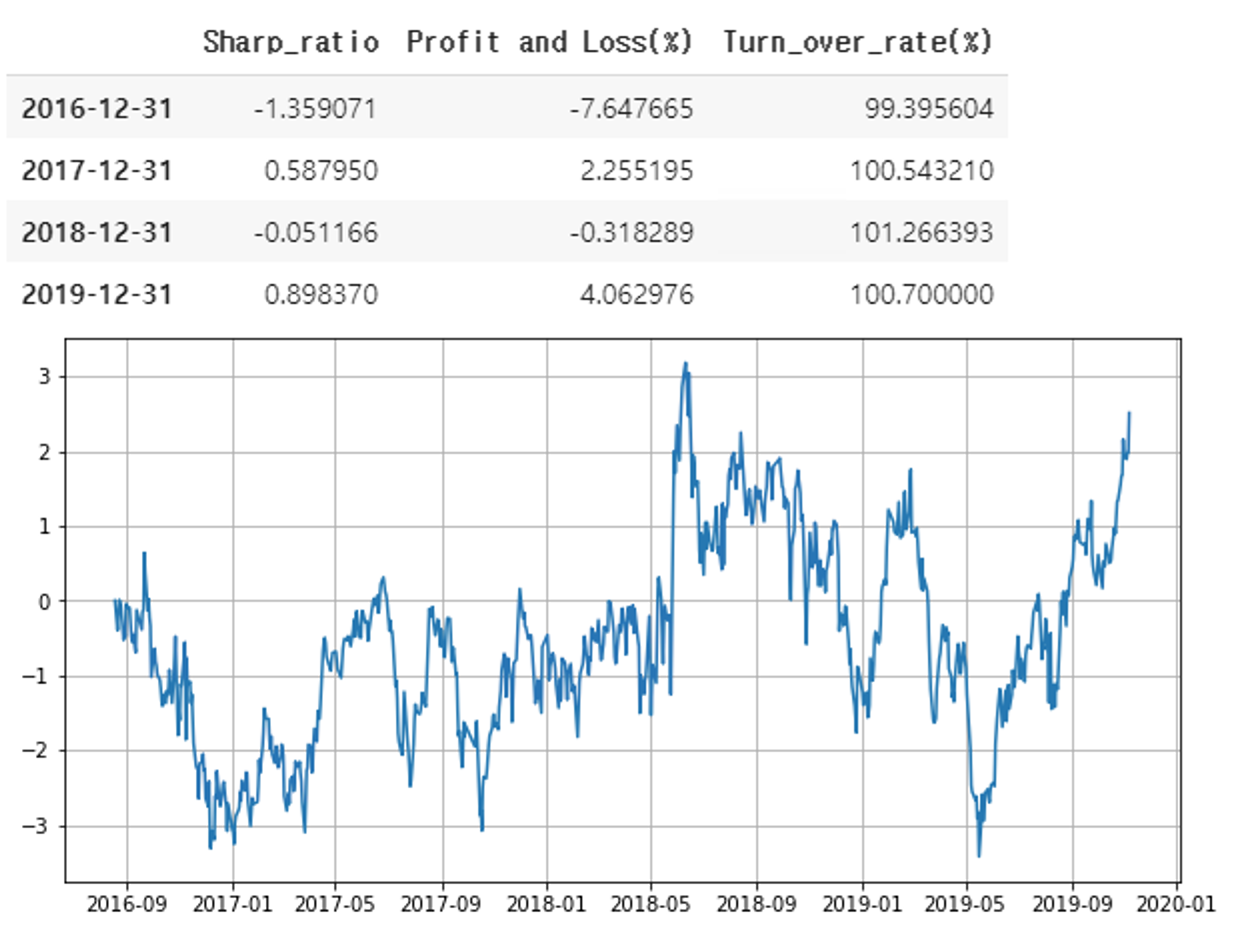
\includegraphics[width=\textwidth/4*3]{images/aaa.png}
    \caption{Performance of the mean-reversion strategy when $\alpha= 0.5$, with other parameters fixed.}
    \label{bigalpha}
    \vspace*{-5mm}
\end{figure}

\begin{figure}
    \centering
    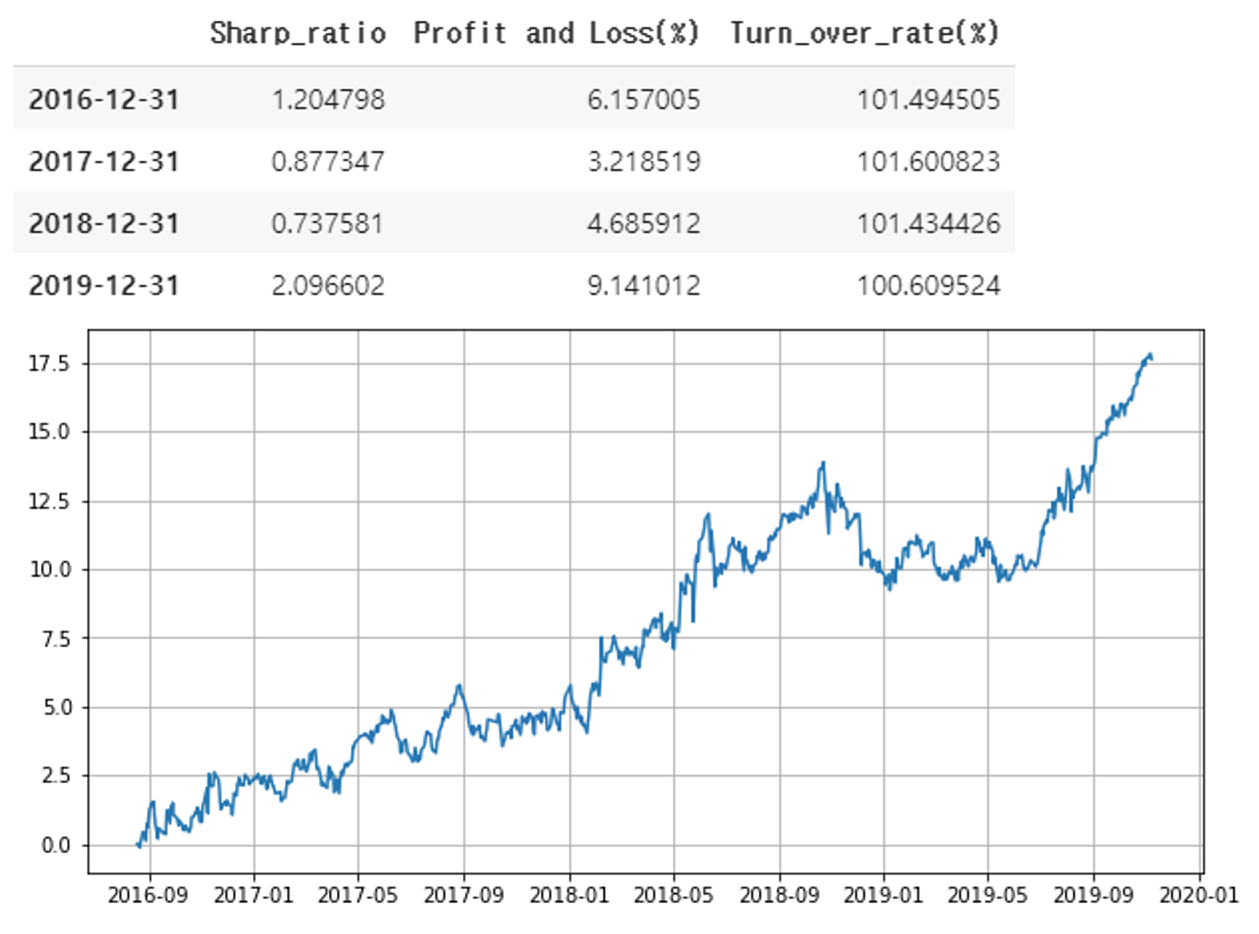
\includegraphics[width=\textwidth/4*3]{images/bbb.png}
    \caption{Result of the mean-reversion strategy when $n$ = 200, $d = 5$, and $c$ = 10.}
    \label{deep result 1}
    \vspace*{-5mm}
\end{figure}

\begin{figure}
    \centering
    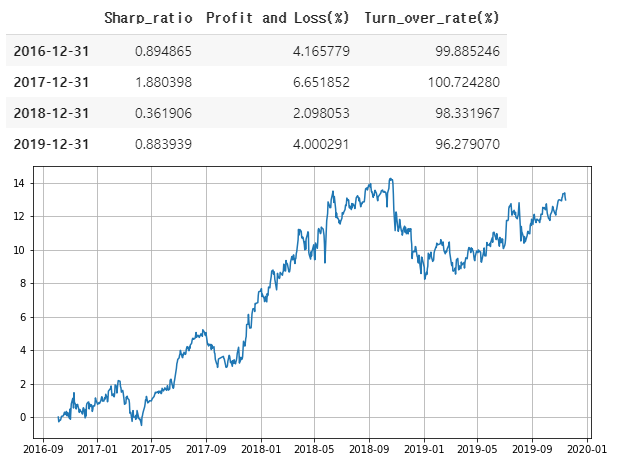
\includegraphics[width=\textwidth/4*3]{images/capt.png}
    \caption{Result of the mean-reversion strategy when $n$ = 500, $d = 5$, and $c$ = 20.}
    \label{deep result 2}
    \vspace*{-5mm}
\end{figure}

\begin{figure}
    \centering
    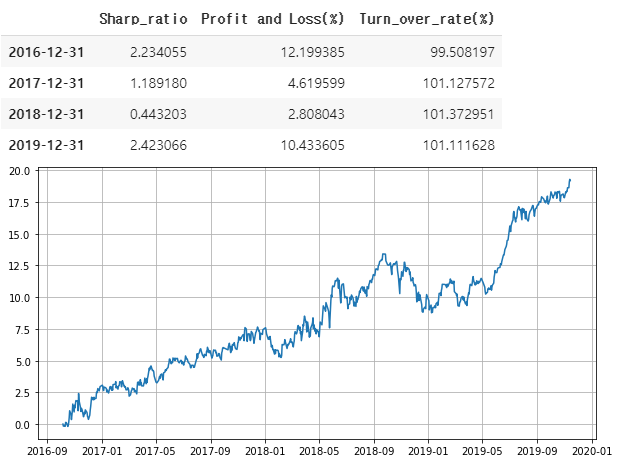
\includegraphics[width=\textwidth/4*3]{images/capt2.png}
    \caption{Result of the mean-reversion strategy when $n$ = 500, $d = 30$, and $c$ = 20, with double the training time.}
    \label{deep result 3}
    \vspace*{-5mm}
\end{figure}





\end{document}
